\chapter{Implementation}\label{Implementation}
\begin{figure}
    \centering
    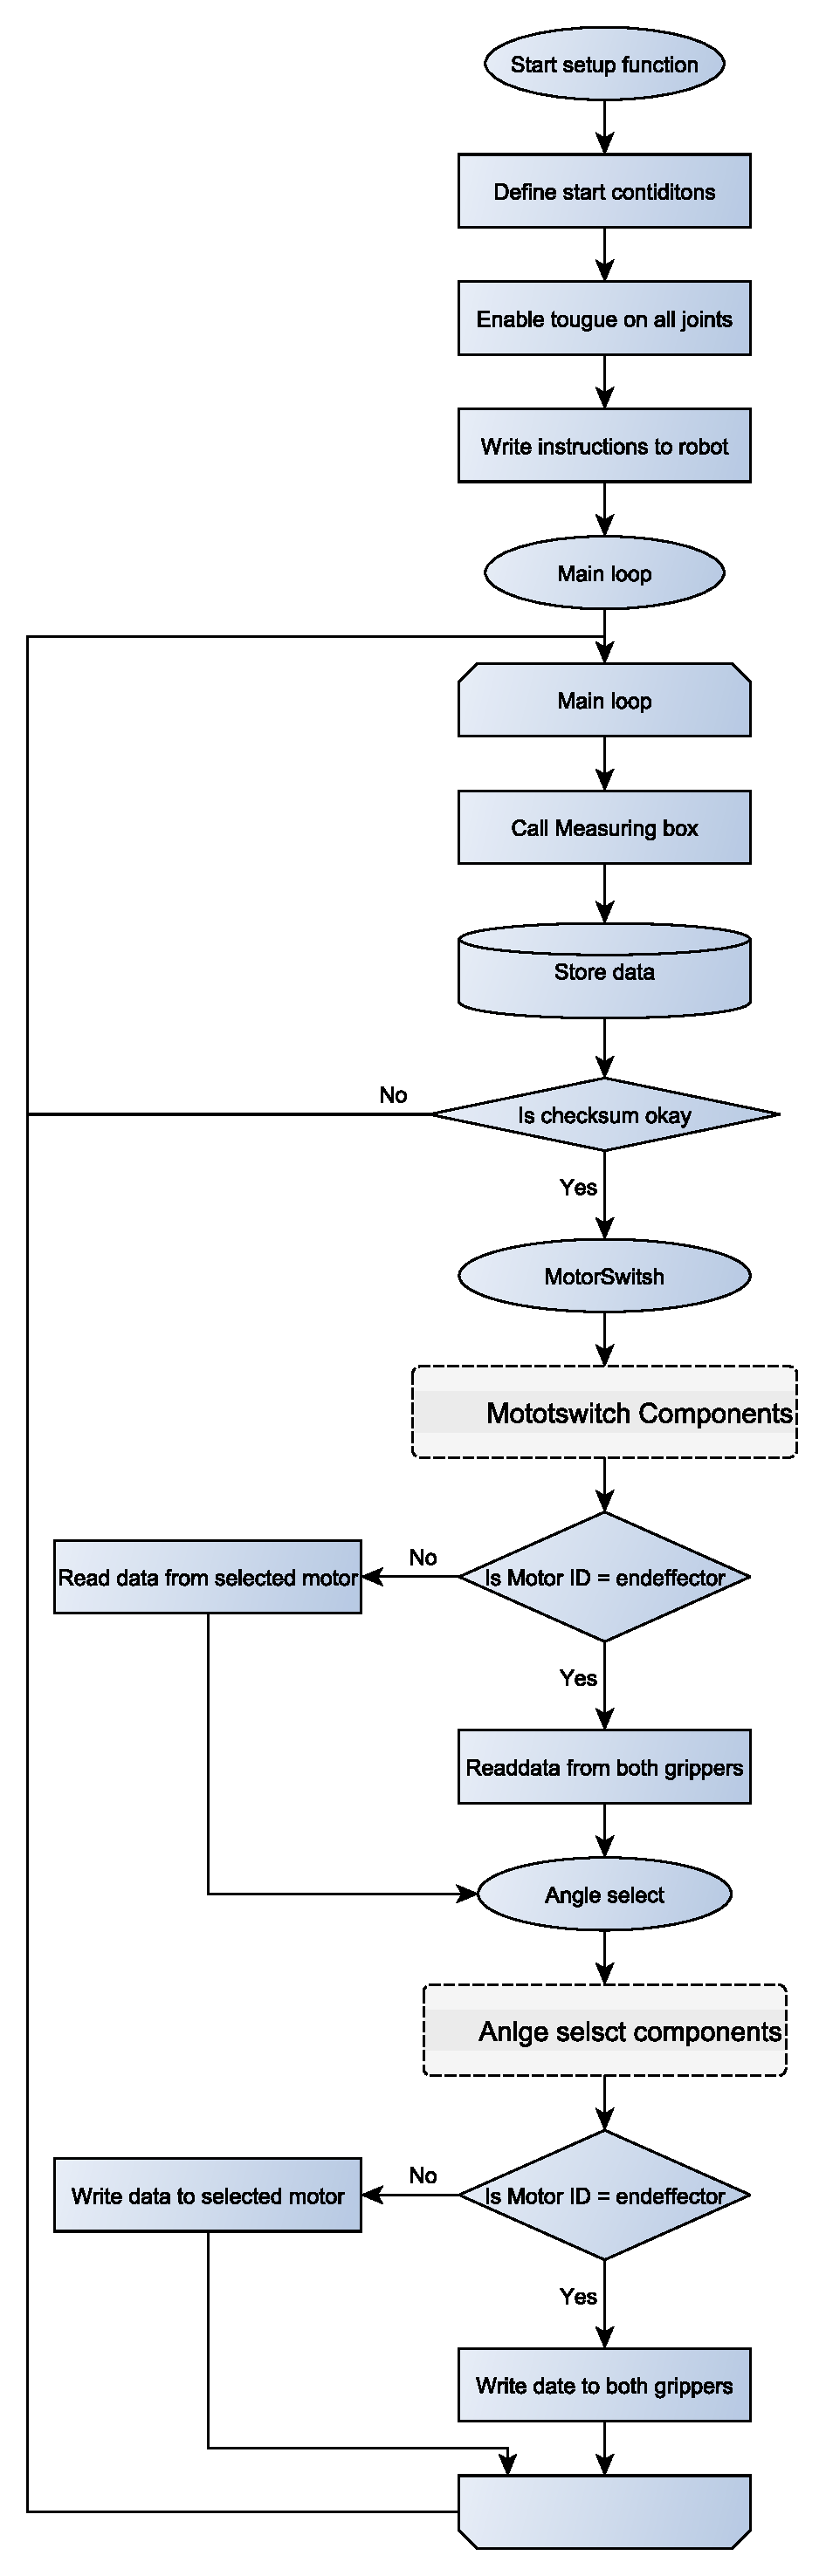
\includegraphics[width=0.5\textwidth]{Figures/Technical_figures/Smallerflowchart.pdf}
    \caption{Flowchart of the code used in this project}
    \label{fig:my_label}
\end{figure}

\section{SW implementation}
\subsubsection{ MotorSwitch }
\begin{figure}[H]
    \centering
    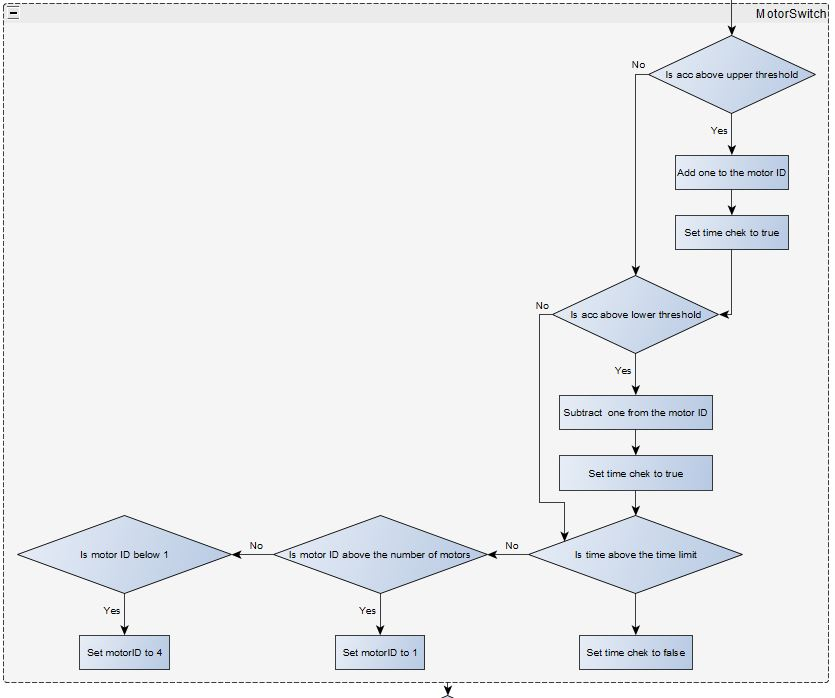
\includegraphics[width=\textwidth]{Figures/Technical_figures/Motor_select_flow.JPG}
    \caption{Caption}
    \label{fig:my_label}
\end{figure}
As shown below the code of switching the motors is presented. This code is a function implemented to control the signals of the accelerometer. This code makes use of the Z-axis, which is the the axis it is meant to operate in when the user lifts the shoulder.\\

\begin{figure}[H]
    \centering
\begin{lstlisting}[frame=single,language=Arduino] 
void MotorSwitch(int &MotorNR, int DD,bool &timeCehk,unsigned long &Time){
    if (DD>800 && timeCehk==false){
        MotorNR = MotorNR + 1;
        timeCehk=true;
        Time = millis();
    }
     if (DD < 450 && timeCehk==false){
        MotorNR = MotorNR - 1;
        timeCehk=true;
        Time = millis();
    }
    if (millis() - Time >= 300){
      timeCehk=false;
    }
    if (MotorNR > 4){
        MotorNR = 1;
    }
     if (MotorNR < 1){
        MotorNR = 4;
    } 
    else{}
 }
\end{lstlisting}
    \caption{Motor Selection, a function written in Arduino code}
    \label{fig:motorSel}
\end{figure}

In line 1, an initialisation is commenced with the variables it is wished to use.\\
At Line 2 and 7, two different if statements is produced. The statements only run if DD is over 800, and if timecheck is false. DD is the accelerometers Z-axis acceleration. Timechek is always false unless a if statement is run as seen in line 4 and 9.\\
MotorNR has a pre-set of 1, which means it is set to motor 1. When the different if statements is run the motor will switch respectively to the if statements.\\
Line 12 consists of the current time and the time passed, which has to be more or equal to 3 seconds. timecheck will then be set to false so the if statements can be run again.\\
The last lines of code is simply to keep the motors from exceeding the number of motors available.

\subsubsection{Angleselect}
\begin{figure}[H]
    \centering
    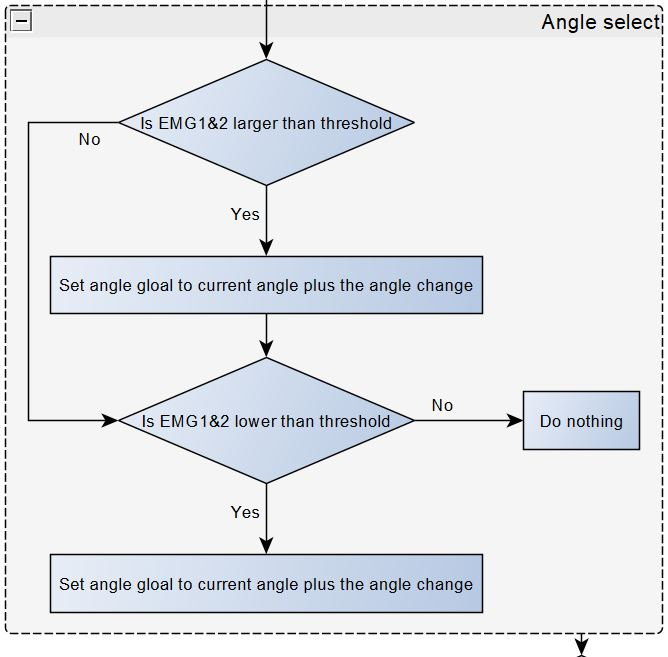
\includegraphics[width=\textwidth]{Figures/Technical_figures/Anlge_select_flow.JPG}
    \caption{Flowchart of the }
    \label{fig:my_label}
\end{figure}
AngleSelect is a function that increases or decreases the angle of the manipulator. This makes the manipulator more manoeuvrable and easy to steer for the user.\\
\begin{figure}[H]
    \centering
   


\begin{lstlisting}[frame=single,language=Arduino]
void AngleSelect(int32_t &ArrNow, int &MotorNR, int &ArrGoal, int EMG_1, int EMG_2, int32_t &PWM, bool &on){
  int thredH = 50;
  int thredL = 50;
  int AngleChange = 10;
  if (MotorNR == 1){
    if (EMG_1 >= thredH && EMG_2 <= thredL){
      ArrGoal = ArrGoal + AngleChange;
      PWM = 360;
      on = true;
    }
    else if (EMG_2 >= thredH && EMG_1 <= thredL){
      ArrGoal = ArrGoal - AngleChange;
      PWM = 360;
      on = true;
    }
    else{
      if (on == true){
        ArrGoal = ArrNow;
      }
      on = false;
    }
  }
  else{
    if (EMG_1 >= thredH && EMG_2 <= thredL){
      ArrGoal = ArrGoal + AngleChange;
      PWM = 360;
      on = true;
    }
    else if (EMG_2 >= thredH && EMG_1 <= thredL){
      ArrGoal = ArrGoal - AngleChange;
      PWM = 262;
      on = true;
    }
    else{
      if (on == true){
        ArrGoal = ArrNow;
        on = false;
      }
    }
  }
  return;
};
\end{lstlisting} \label{fig:AS}


    \caption{Angle Selection, a function written in Arduino code}
    \label{fig:AngleSel}
\end{figure}
Line one consists of the function and its parameters, where ArrNow is the angle which the manipulator is in, and ArrGoal is which angle is desired of the user.\\
In line 2 AngleChange is set to 6, which will be used in line 4.\\
Line 3 is a if statement with two parameters that has to be true, EMG1 must be over or equal to 300 and EMG2 must be lower or equal to 50. When this statement is run a simple equation will begin, which adds ArrNow and the AngleChange together, to move the motor. Line 6 and 7 is simply the same but reversed, so it is possible that the AngleChange can be retracted to move the motor the opposite direction. 

\subsection{CheckSum and checksum verification}
The Checksum Method is used to ensure the transmitted date hasnot been corrupted or disrupted.
\paragraph{Checksum:}In the Xbee byte array(24Bytes), in see fig:\ref{fig:XbeeDataFromOldSolution}, the checksum is the last byte in the array.\\
\begin{figure}[H]
 \centering 
    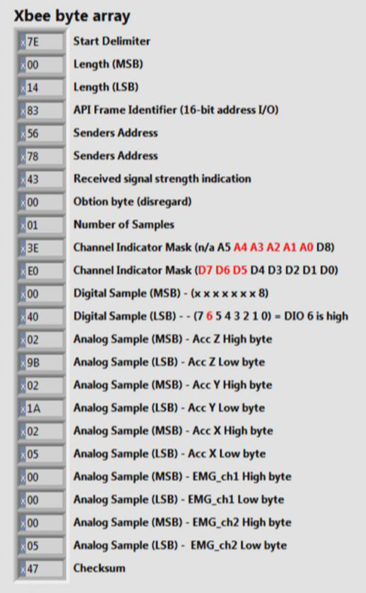
\includegraphics[scale=0.7]{Figures/EMG/XbeeDataArray.png}
    \caption{How the bytes in the Xbee Byte array, is structured}
    \label{fig:XbeeDataFromOldSolution}
\end{figure}
The bytes excluding the Start delimiter, the Length bytes and the checksum is referred to at the API-specific structure. 
The Xbee checksum is calculated by adding all the bytes in the API-specific structure, keeping only the 8 lowest bits in the result and subtracting it from 0xFF in hexadecimal(255 in Decimal)\cite{Calculat82:online}.
\paragraph{Checksum Verification:}
The sum of the API-specific structure with the transmitted checksum added is 0xFF, if the transmission has not been altered. As such the verification is done by verifying this.

\subsubsection{Code explanation}
 \begin{lstlisting}[frame=single,language=Arduino] 
void emgCom(int &sumx, int &sumy, int &sumz, int &sumemg1, int &sumemg2 ) {
  byte disbyte[22];
  bool chkRec = false;
  while (chkRec == false) {
    if (Serial2.available() >= 24) {
      if (Serial2.read() == 126) {
        for (int i = 0; i <= 22; i++) {
          disbyte[i] = Serial2.read();
        }
        int chkSum = 0;
        for (int i = 2; i <= 22; i++) {
          chkSum = chkSum + disbyte[i];
        }
        if (lowByte(chkSum) == 0xFF) {
          sumz = disbyte[13] + (disbyte[12] * 256);
          sumy = disbyte[15] + (disbyte[14] * 256);
          sumx = disbyte[17] + (disbyte[16] * 256);
          sumemg1 = disbyte[19] + (disbyte[18] * 256);
          sumemg2 = disbyte[21] + (disbyte[20] * 256);
          if( sumemg1<=1024 && sumemg2 <=1024 ){
          chkRec = true;
          }
          else{}
        }
      }
    }
  }
  return;
}
\end{lstlisting}\label{CheckSumCode}
\paragraph{Line 2-9}Firstly, the array \textit{disbyte[22]} is made.
Then the teensy search the data from the Xbee to look for the start delimiter which is 126 or 0x7E and stores the next 23 of bytes.
\paragraph{Line 10-13:}The int \textit{chkSum} is the sum of the API-specific structure and the checksum byte. It is calculated by adding up the the bytes in the disbyte[22] array excluding the two length bytes from the Xbee.

\paragraph{Line 14-19}The \textit{chkSum} value is tested to ensure it has the value 0xFF. Then sum z, sum y, sum x, sum emg1 and sum emg2 are calculated to be used in the for data.


\paragraph{Line 20} Due to that the \textit{chkSum} in some instances can be 255 without being altered. One more check than the check sum done through the \textit{if} statement where if the EMG signal is above 1024 then \textit{chkRec} will not be set true. This will keep the loop running till it as a correct packet.
\subsubsection{Control algorithm}


%\subsubsection{Communication protocol}
%Communication between the PC and the Teensy is setup so that the Teensy have to receive a string. The string have to contain an AB at the beginning and at the end DC and a newline character $'\backslash n'$. As a delimiter for the string the choice fell on $'\colon'$ a colon, so for each joint there is send a value to give a goal position and and a movement speed. The packet is has to have this form:\\
\begin{center}
     AB\colon$joint_1$ goal\colon$joint_1$ speed\colon$joint_2$ goal\colon$joint_2$ speed\colon$joint_3$ goal\colon$joint_3$ speed\\\colon$joint_4$ goal\colon$joint_4$ speed\colon$joint_5$ goal\colon$joint_5$ speed\colon DC\colon$\backslash n$   \\
    
\end{center}
   
When the Teensy receives the message it checks for the AB characters, if they are found, it processes each value and stores temporarily, at the end it checks for DC and if these characters are there as well the Teensy will store the values properly. \\
The feedback communication from the Teensy to the PC is send with the delimiter of ' ' a white space, when the Matlab program receives the message through serial port it will store the values in an array that takes this form:\\
 \begin{center}
     \emph{The converted message in Matlab from the Teensy}\\
     $10 \times 1$~array
 \end{center}

\[ \left( \begin{array}{c}
Joint_1 \mbox{ current position}   \\
Joint_1 \mbox{ current velocity}  \\
Joint_2 \mbox{ current position}   \\
Joint_2 \mbox{ current velocity}  \\
Joint_3 \mbox{ current position}   \\
Joint_3 \mbox{ current velocity}  \\
Joint_4 \mbox{ current position}   \\
Joint_4 \mbox{ current velocity}  \\
Joint_5 \mbox{ current position}   \\
Joint_5 \mbox{ current velocity}
\end{array} \right)\] \\

All data points can then be used in the feedback control part for the prostheses. 


%subsection{Communication between Teensy and CrustCrawler}
\section{HW implementation}
\subsection*{Wire connection}
\begin{figure}[H]
    \centering
\tikzset{every picture/.style={line width=0.75pt}} %set default line width to 0.75pt        

\begin{tikzpicture}[x=0.75pt,y=0.75pt,yscale=-1,xscale=1]
%uncomment if require: \path (0,374); %set diagram left start at 0, and has height of 374

%Image [id:dp7152221511204973] 
\draw (269.48,152.73) node  {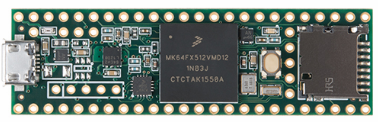
\includegraphics[width=197.45pt,height=60.59pt]{Figures/TikzFigures/layOut/teensy.PNG}};
%Image [id:dp37486105933332636] 
\draw (366.16,279.14) node [rotate=-180.22,xslant=-0.01] {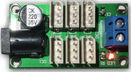
\includegraphics[width=89.36pt,height=69.95pt]{Figures/TikzFigures/layOut/supl.PNG}};
%Image [id:dp9034481830242995] 
\draw (132.79,272.76) node [rotate=-359.65,xslant=0] {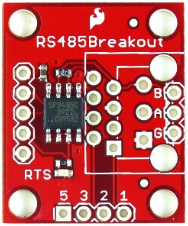
\includegraphics[width=83.35pt,height=72.71pt]{Figures/TikzFigures/layOut/rs.PNG}};
%Image [id:dp11028803786694708] 
\draw (236.5,45.39) node [rotate=-270] {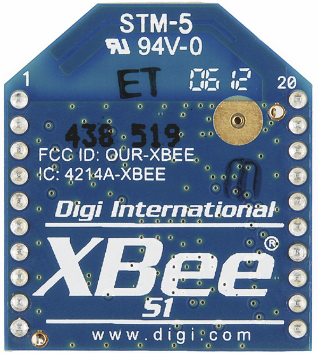
\includegraphics[width=60.59pt,height=62.4pt]{Figures/TikzFigures/layOut/bee.PNG}};
%Left Arrow [id:dp5012443384308891] 
\draw   (438.55,274.06) -- (457.33,256.75) -- (457.33,265.41) -- (485.5,265.41) -- (485.5,282.72) -- (457.33,282.72) -- (457.33,291.38) -- cycle ;
%Right Arrow [id:dp0023557246216043826] 
\draw   (80.2,146.67) -- (111.93,146.67) -- (111.93,137.72) -- (133.09,155.61) -- (111.93,173.5) -- (111.93,164.56) -- (80.2,164.56) -- cycle ;
%Straight Lines [id:da08227247794525927] 
\draw [color={rgb, 255:red, 247; green, 10; blue, 10 }  ,draw opacity=1 ][line width=1.5]    (150.92,81.17) -- (150.52,123.87) ;


%Straight Lines [id:da025924835708441174] 
\draw [color={rgb, 255:red, 247; green, 10; blue, 10 }  ,draw opacity=1 ][line width=1.5]    (217.48,81.17) -- (150.92,81.17) ;


%Straight Lines [id:da00602413999639384] 
\draw [color={rgb, 255:red, 247; green, 10; blue, 10 }  ,draw opacity=1 ][line width=1.5]    (42.76,80.79) -- (155.28,80.79) ;


%Straight Lines [id:da7149252935730617] 
\draw [color={rgb, 255:red, 247; green, 10; blue, 10 }  ,draw opacity=1 ][line width=1.5]    (43.55,80.79) -- (43.55,256.21) ;


%Straight Lines [id:da3829700368795059] 
\draw [color={rgb, 255:red, 247; green, 10; blue, 10 }  ,draw opacity=1 ][line width=1.5]    (91.09,256.21) -- (43.55,256.21) ;


%Straight Lines [id:da8981864779638247] 
\draw [line width=1.5]    (31.67,88.48) -- (31.67,290.84) ;


%Straight Lines [id:da6466608797084847] 
\draw [line width=1.5]    (91.89,290.07) -- (31.67,290.07) ;


%Straight Lines [id:da35185368144106244] 
\draw [line width=1.5]    (31.67,88.48) -- (272.55,89.25) ;


%Straight Lines [id:da8387196090383506] 
\draw    (271.76,80.02) -- (271.76,89.25) ;


%Straight Lines [id:da36845317589148996] 
\draw [color={rgb, 255:red, 91; green, 235; blue, 46 }  ,draw opacity=1 ][line width=1.5]    (225.01,81.56) -- (160.03,184.66) ;


%Straight Lines [id:da4171143722401429] 
\draw [color={rgb, 255:red, 248; green, 231; blue, 28 }  ,draw opacity=1 ][line width=1.5]    (231.55,81.56) -- (173.71,184.66) ;


%Straight Lines [id:da33656991606038633] 
\draw [color={rgb, 255:red, 32; green, 240; blue, 26 }  ,draw opacity=1 ][line width=1.5]    (90.3,273.91) -- (265.42,185.43) ;


%Straight Lines [id:da3740974102672152] 
\draw [color={rgb, 255:red, 244; green, 250; blue, 27 }  ,draw opacity=1 ][line width=1.5]    (255.91,184.66) -- (91.89,265.45) ;


%Straight Lines [id:da18281067478913027] 
\draw [color={rgb, 255:red, 74; green, 144; blue, 226 }  ,draw opacity=1 ][line width=1.5]    (91.09,282.37) -- (276.51,185.43) ;


%Straight Lines [id:da7137403407481466] 
\draw [line width=1.5]    (180.34,279.84) -- (343.47,319.08) ;


%Straight Lines [id:da9319303523938192] 
\draw [color={rgb, 255:red, 243; green, 20; blue, 20 }  ,draw opacity=1 ][line width=1.5]    (180.34,271.18) -- (344.5,305) ;


%Straight Lines [id:da7229658725423573] 
\draw [color={rgb, 255:red, 74; green, 144; blue, 226 }  ,draw opacity=1 ][line width=1.5]    (180.34,262.52) -- (343.5,296) ;


%Straight Lines [id:da43545523008986176] 
\draw [line width=1.5]    (31.5,202) -- (150.5,202) ;


%Straight Lines [id:da5107595655280059] 
\draw [line width=1.5]    (150.5,183) -- (150.5,202) ;



% Text Node
\draw (99.41,156.19) node  [align=left] {USB};
% Text Node
\draw (465.49,273.68) node  [align=left] {12V};
% Text Node
\draw (77,191) node  [align=left] {Gnd};
% Text Node
\draw (98,71) node  [align=left] {5V};
% Text Node
\draw (257,310) node  [align=left] {Gnd};
% Text Node
\draw (263,265) node  [align=left] {Rs 485};
% Text Node
\draw (338,106) node  [align=left] {Teensy 3.5};
% Text Node
\draw (133,341) node  [align=left] { \ \ \ BOB-10124\\Rs 232 to Rs 485};

% Text Node
\draw (212,108) node  [align=left] {Rx1 \ \ \ Tx1};
% Text Node
\draw (192,199) node  [align=left] {RxTx2};
% Text Node
\draw (317,212) node  [align=left] {Transmit enable wire};


\end{tikzpicture}
    \caption{Wiring of the Teensy to external components}
    \label{fig:motorSel}
\end{figure}
\subsection*{sEMG placement}
\begin{figure}[H]
    \centering       
\tikzset{every picture/.style={line width=0.75pt}} %set default line width to 0.75pt        

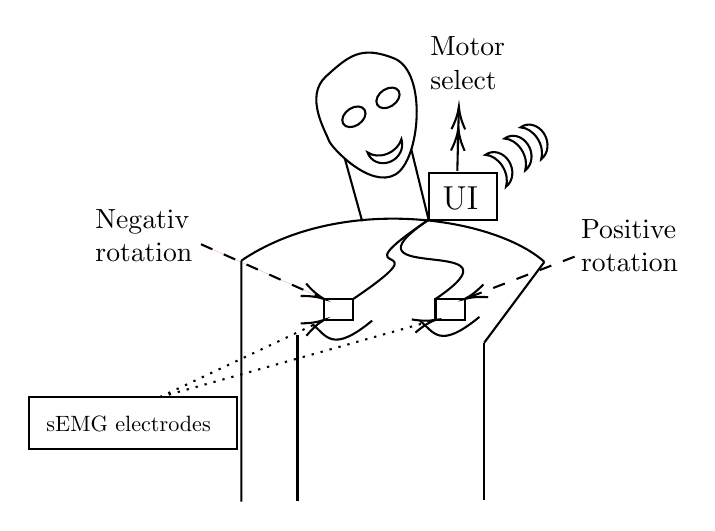
\begin{tikzpicture}[x=0.75pt,y=0.75pt,yscale=-1,xscale=1]
%uncomment if require: \path (0,348.6666564941406); %set diagram left start at 0, and has height of 348.6666564941406

%Straight Lines [id:da48983191890161915] 
\draw    (302.93,184.24) -- (302.95,300.29) ;


%Straight Lines [id:da551487490016626] 
\draw    (330,220) -- (330,300) ;


%Straight Lines [id:da6135134184778834] 
\draw    (419.95,223.79) -- (419.95,299.79) ;


%Curve Lines [id:da40002913632145076] 
\draw    (337.25,214.92) .. controls (344.01,220.3) and (346.39,229.26) .. (365.97,213.14) ;


%Curve Lines [id:da017442708579094912] 
\draw    (388.93,213.13) .. controls (395.68,218.5) and (398.07,227.47) .. (417.65,211.35) ;


%Shape: Rectangle [id:dp2948369463848257] 
\draw   (342.82,202.73) -- (356.83,202.73) -- (356.83,212.78) -- (342.82,212.78) -- cycle ;
%Shape: Rectangle [id:dp8177370839769769] 
\draw   (396.48,202.73) -- (410.49,202.73) -- (410.49,212.78) -- (396.48,212.78) -- cycle ;
%Shape: Polygon Curved [id:ds39308421777793057] 
\draw   (343.78,95.42) .. controls (354.51,85.74) and (360.48,80.36) .. (376.58,86.82) .. controls (392.67,93.27) and (389.17,135.74) .. (377.17,142.74) .. controls (365.18,149.74) and (346.17,129.83) .. (344.97,126.07) .. controls (343.78,122.31) and (333.05,105.1) .. (343.78,95.42) -- cycle ;
%Curve Lines [id:da9166271647364232] 
\draw    (302.93,184.24) .. controls (350.63,151.98) and (424.5,162.97) .. (448.95,184.83) ;


%Straight Lines [id:da6940855715795691] 
\draw    (352.82,135.14) -- (361.17,165.25) ;


%Straight Lines [id:da06557587996091874] 
\draw    (384.85,130.69) -- (393.16,164.56) ;


%Shape: Rectangle [id:dp44542314487649004] 
\draw   (393.16,141.97) -- (426.16,141.97) -- (426.16,164.56) -- (393.16,164.56) -- cycle ;
%Straight Lines [id:da5886591469978335] 
\draw    (448.95,184.83) -- (419.95,223.79) ;


%Curve Lines [id:da438028737656337] 
\draw    (356.83,202.73) .. controls (404.53,170.47) and (345.46,196.83) .. (393.16,164.56) ;


%Curve Lines [id:da298231790072667] 
\draw    (396.48,202.73) .. controls (444.18,170.47) and (345.46,196.83) .. (393.16,164.56) ;


%Straight Lines [id:da17698811288515226] 
\draw  [dash pattern={on 0.84pt off 2.51pt}]  (263.68,250.01) -- (341.01,213.63) ;
\draw [shift={(342.82,212.78)}, rotate = 514.81] [color={rgb, 255:red, 0; green, 0; blue, 0 }  ][line width=0.75]    (10.93,-3.29) .. controls (6.95,-1.4) and (3.31,-0.3) .. (0,0) .. controls (3.31,0.3) and (6.95,1.4) .. (10.93,3.29)   ;

%Straight Lines [id:da4704201066732616] 
\draw  [dash pattern={on 0.84pt off 2.51pt}]  (263.68,250.01) -- (394.55,213.32) ;
\draw [shift={(396.48,212.78)}, rotate = 524.3399999999999] [color={rgb, 255:red, 0; green, 0; blue, 0 }  ][line width=0.75]    (10.93,-3.29) .. controls (6.95,-1.4) and (3.31,-0.3) .. (0,0) .. controls (3.31,0.3) and (6.95,1.4) .. (10.93,3.29)   ;

%Shape: Rectangle [id:dp09154428052258479] 
\draw   (200.5,249.85) -- (300.86,249.85) -- (300.86,274.77) -- (200.5,274.77) -- cycle ;
%Shape: Moon [id:dp8725784672937908] 
\draw   (420.51,133.29) .. controls (423.99,130.68) and (429.04,131.98) .. (431.79,136.21) .. controls (434.54,140.43) and (433.95,145.98) .. (430.48,148.6) .. controls (431.36,145.65) and (430.77,141.85) .. (428.64,138.58) .. controls (426.51,135.31) and (423.39,133.4) .. (420.51,133.29) -- cycle ;
%Shape: Moon [id:dp39582079060737096] 
\draw   (429.75,125.43) .. controls (433.23,122.81) and (438.27,124.11) .. (441.03,128.34) .. controls (443.78,132.56) and (443.19,138.11) .. (439.71,140.73) .. controls (440.6,137.79) and (440.01,133.98) .. (437.88,130.71) .. controls (435.75,127.44) and (432.63,125.54) .. (429.75,125.43) -- cycle ;
%Shape: Moon [id:dp049975679573210696] 
\draw   (437.45,120.04) .. controls (440.92,117.42) and (445.97,118.73) .. (448.72,122.95) .. controls (451.48,127.18) and (450.89,132.73) .. (447.41,135.35) .. controls (448.3,132.4) and (447.71,128.59) .. (445.58,125.33) .. controls (443.45,122.06) and (440.33,120.15) .. (437.45,120.04) -- cycle ;
%Shape: Moon [id:dp9195347803104288] 
\draw   (380.06,125.7) .. controls (381.51,129.99) and (379.03,134.9) .. (374.53,136.66) .. controls (370.02,138.43) and (365.19,136.38) .. (363.74,132.09) .. controls (366.15,133.77) and (369.73,134.14) .. (373.21,132.78) .. controls (376.7,131.41) and (379.22,128.66) .. (380.06,125.7) -- cycle ;
%Shape: Ellipse [id:dp8827523909159829] 
\draw   (362.38,111.69) .. controls (363.5,113.77) and (362.07,116.91) .. (359.19,118.7) .. controls (356.31,120.49) and (353.06,120.25) .. (351.95,118.17) .. controls (350.83,116.09) and (352.27,112.96) .. (355.15,111.17) .. controls (358.03,109.38) and (361.27,109.61) .. (362.38,111.69) -- cycle ;
%Shape: Ellipse [id:dp42511842093367047] 
\draw   (378.81,102.58) .. controls (379.92,104.66) and (378.49,107.79) .. (375.61,109.58) .. controls (372.73,111.38) and (369.49,111.14) .. (368.37,109.06) .. controls (367.26,106.98) and (368.69,103.85) .. (371.57,102.06) .. controls (374.45,100.27) and (377.69,100.5) .. (378.81,102.58) -- cycle ;
%Straight Lines [id:da8820566539783692] 
\draw    (407,141) -- (407.45,122.33) ;
\draw [shift={(407.5,120.33)}, rotate = 451.39] [color={rgb, 255:red, 0; green, 0; blue, 0 }  ][line width=0.75]    (10.93,-3.29) .. controls (6.95,-1.4) and (3.31,-0.3) .. (0,0) .. controls (3.31,0.3) and (6.95,1.4) .. (10.93,3.29)   ;

%Straight Lines [id:da5478933045813028] 
\draw    (407.25,130.67) -- (407.7,112) ;
\draw [shift={(407.75,110)}, rotate = 451.39] [color={rgb, 255:red, 0; green, 0; blue, 0 }  ][line width=0.75]    (10.93,-3.29) .. controls (6.95,-1.4) and (3.31,-0.3) .. (0,0) .. controls (3.31,0.3) and (6.95,1.4) .. (10.93,3.29)   ;

%Straight Lines [id:da9326088231862386] 
\draw [fill={rgb, 255:red, 216; green, 21; blue, 21 }  ,fill opacity=1 ] [dash pattern={on 4.5pt off 4.5pt}]  (283.5,176.33) -- (340.99,201.92) ;
\draw [shift={(342.82,202.73)}, rotate = 203.99] [color={rgb, 255:red, 0; green, 0; blue, 0 }  ][line width=0.75]    (10.93,-3.29) .. controls (6.95,-1.4) and (3.31,-0.3) .. (0,0) .. controls (3.31,0.3) and (6.95,1.4) .. (10.93,3.29)   ;

%Straight Lines [id:da06992380639248452] 
\draw  [dash pattern={on 4.5pt off 4.5pt}]  (463.5,182.33) -- (412.36,202.01) ;
\draw [shift={(410.49,202.73)}, rotate = 338.95] [color={rgb, 255:red, 0; green, 0; blue, 0 }  ][line width=0.75]    (10.93,-3.29) .. controls (6.95,-1.4) and (3.31,-0.3) .. (0,0) .. controls (3.31,0.3) and (6.95,1.4) .. (10.93,3.29)   ;


% Text Node
\draw (408.49,154.29) node  [align=left] {{\large UI}};
% Text Node
\draw (248.65,262.63) node [scale=0.8] [align=left] {sEMG electrodes};
% Text Node
\draw (412,89) node  [align=left] {Motor\\select};
% Text Node
\draw (256,172) node  [align=left] {Negativ\\rotation};
% Text Node
\draw (490,177) node  [align=left] {Positive\\rotation};


\end{tikzpicture}


   \caption{Physical setup of control}
    \label{fig:PCS}
\end{figure}



